\documentclass[11pt]{book}

\usepackage{titlepic}
\usepackage{graphicx} % Required for inserting images

\title{1° Relatório: Projeto ULA de 8 operações}
\author{\textbf{Anna Luisa de Sá dos Santos}(DRE: 121050671),\\ \textbf{Larissa Rocha dos Santos}(DRE: 121072380 ),\\ \textbf{Reginaldo da Silva Cardoso Santos}(DRE: 121039544).\\}

\date{\today}

\titlepic{
\includegraphics[width=50mm,scale=0.5]{UFRJicon.png}}

\begin{document}
    \maketitle
    \frontmatter
    \renewcommand*\contentsname{Sumário}
    \tableofcontents

\chapter{Introdução}
    \section{Apresentação}
    A Unidade Lógica e Aritmética (ULA) é um componente fundamental em diversos sistemas digitais, desempenhando um papel crucial na execução de operações lógicas e aritméticas essenciais para o funcionamento de processadores e outros dispositivos. Este trabalho tem como objetivo desenvolver uma ULA de 4 bits capaz de realizar oito operações distintas, atendendo a requisitos específicos de um ambiente de hardware baseado no Kit Xilinx Spartan3.
    
    \section{Objetivos:}
    Como já citado, o trabalho tem como objetivo desenvolver uma Unidade Lógica e Aritmética (ULA) de 4 bits e com 8 operações. 
    Sob este viés, o grupo optou por realizar a ULA com as operações lógicas'AND', 'NAND', 'OR', 'NOR', 'XOR' e 'XNOR', oferecendo uma gama completa de possibilidades para manipulação de bits. No âmbito aritmético, a ULA incluirá um somador e um subtrator com complemento de 2, que é uma técnica amplamente utilizada em sistemas digitais para simplificar a representação e manipulação de números negativos.
    
    \section{Requisitos:}
    Os requisitos do projeto especificam que a operação da ULA será selecionada por meio de chaves disponíveis no Kit Xilinx Spartan3, garantindo a interatividade e controle direto sobre as funções executadas. Além disso, os dados de entrada serão gerados por um módulo auxiliar denominado “bancada de testes”, o que facilita a verificação e validação das operações da ULA. Os resultados das operações serão exibidos em binário através de um conjunto de 8 LEDs no Kit Xilinx Spartan3, proporcionando uma visualização clara e direta do processamento realizado.

    As saídas da ULA incluirão, além do resultado da operação, quatro flags: Zero, Negativo, Carry out e Overflow. Estes indicadores são fundamentais para a detecção das condições especiais durante as operações, como a ocorrência de um resultado zero, um resultado negativo, um estouro no bit de transporte e um estouro aritmético, respectivamente. Esses elementos são essenciais para a correta operação e controle de sistemas digitais complexos.
    
    Desta forma, os requisitos do trabalho estão de acordo com o exposto abaixo:
        \begin{itemize}
              \item  Operação da ULA selecionada por chaves do Kit Xilinx Spartan3;
              \item Operações obrigatórias: soma e subtração em complemento a 2;
              \item Dados de entrada gerados por um módulo “bancada de testes” auxiliar;
              \item Exibição dos dados em binário no conjunto de 8 LEDs do Kit Xilinx Spartan 3;
              \item Saídas: resultado e 4 flags: Zero, Negativo, Carry out e Overflow.
        \end{itemize}
    
    \chapter{Desenvolvimento}
        \section{Funcionamento :}
        As entradas da ULA são geradas por um módulo “bancada de testes”, parte integrante do projeto. As duas entradas são mostradas sequencialmente nos LEDs de saída. Os LEDS mais à esquerda indicam um código para “entrada A”, “entrada B”, “resultado”, “flags”, em intervalos regulares. Os operandos e o resultado são exibidos nos 4 LEDS mais à direita do kit.
\section{A eletrônica :}
Para realizar o projeto, primeiramente o mesmo foi "rascunhado" utilizando o software "LogiSim Evolution", que permitiu a visualização em alto nível do circuito dada as limitações de Entradas e Saídas da FPGA que eram as seguintes : 
\begin{itemize}
\item 8x LEDS
\item 4x SWITCHES
\item 4x BOTÕES
\end{itemize}
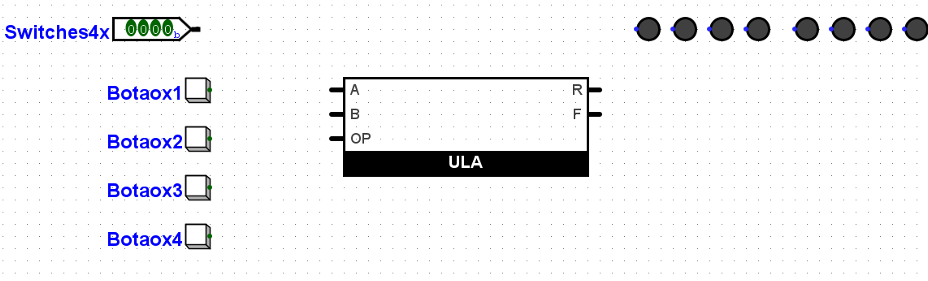
\includegraphics[width=1.2\textwidth]{Design_TopLevel.png}%
Analisando o módulo e os componentes disponíveis, chegamos nas seguintes conclusões: 
\newline
Entradas : 
\begin{itemize}
    \item $A = (A_{3},A_{2},A_{1},A_{0})|A_{i}\in{(0,3)}$
    \item $B = (B_{3},B_{2},B_{1},B_{0})|B_{i}\in{(0,3)}$
    \item $Op = (Op_{2},Op_{1},Op_{0})|Op_{i}\in{(0,2)}$
    \item $Clock\in{(0,1)}$
\end{itemize}
Saídas : 
\begin{itemize}
    \item $Resultado = (R_{7},R_{6},R_{5},R_{4},R_{3},R_{2},R_{1},R_{0})|R_{i}\in{(0,8)}$
\end{itemize}

Modulos necessários : 
\begin{itemize}
    \item Precisamos de um barramento para os switches definirem cada uma das entradas de cada vez. 
    \item Muxes para distribuir à cada LED de maneira organizada o Resultado,Operação,Entrada A e Entrada B.
    \item Um decodificador para selecionar qual das entradas recebe a entrada única.
    \item Registradores pois precisamos que nossas entradas sejam salvas antes de seu transbordo.
    \item Contadores já que apesar da nossa ULA ser combinacional queremos mostrar os valores nos LEDS sincronamente. 
    \item E por fim para evitar problemas físicos e de temporização um circuito de Debounce.
    \item E um circuito capaz de dividir o clock.
\end{itemize}

Organizando o circuito pelo LogiSim, teremos a seguinte configuração : 
\newline\newline
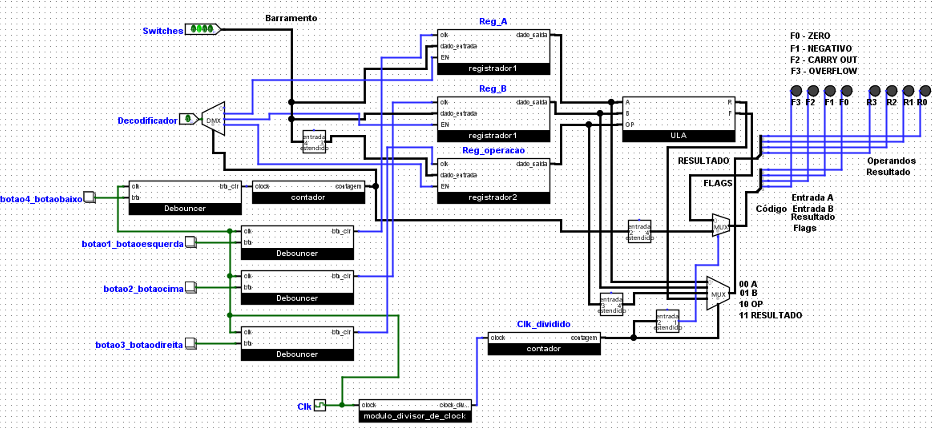
\includegraphics[width=1.2\textwidth]{Design_Completo.png}%
\newline\newline
Com o nosso design de alto nivel pronto, criamos um diagrama de fluxo de dados da seguinte forma : 
\newline\newline
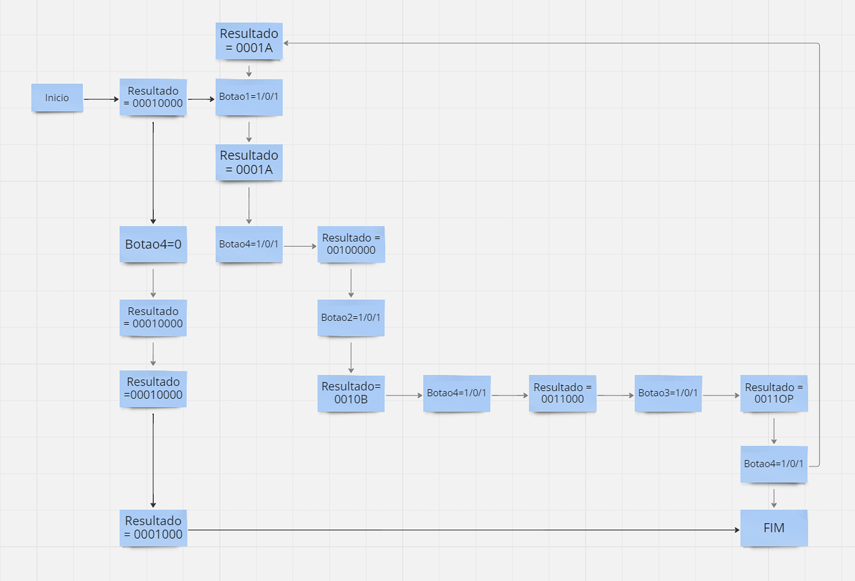
\includegraphics[width=1.1\textwidth]{Diagrama_de_Fluxo.png}%
\newline\newline
Portanto, além do clock da FPGA, utilizaremos botões como o clock dos registradores da nossa bancada de testes. 

\section{O código e simulações : }

Nesta seção visualizaremos os módulos da bancada de teste.
\newline\newline


\textbf{Módulo divisor de Clock :} 
\newline\newline
Para efetuar a divisão do clock de 50mhz fizemos a seguinte operação: 
\newline\newline
Sabemos que $50mhz(50$x$10^{6}s^{-1}) = 20ns$, 
\newline\newline
portanto precisamos dividir o nosso clock de modo que seja possivel visualizar as saidas em no mínimo milissegundos ou segundos, então utilizamos flip-flops divisores que incrementase 1 a cada clock, e utilizamos 26 entradas, portanto:
\newline\newline
2$^{26}$= 67.108.864, 20ns = 2$^{-8}$s, portanto temos um clock de aproximadamente 1,4 segundo, logo que : 
\newline\newline
 Se contamos $1$ em cada 2$^{-8}$ segundo, para determinar quanto tempo levariamos, faremos a seguinte operação : $67.108.864$ x $0,00000002s = 1,34s$
\newline\newline
O código VHDL fica da seguinte forma :
\newline\newline
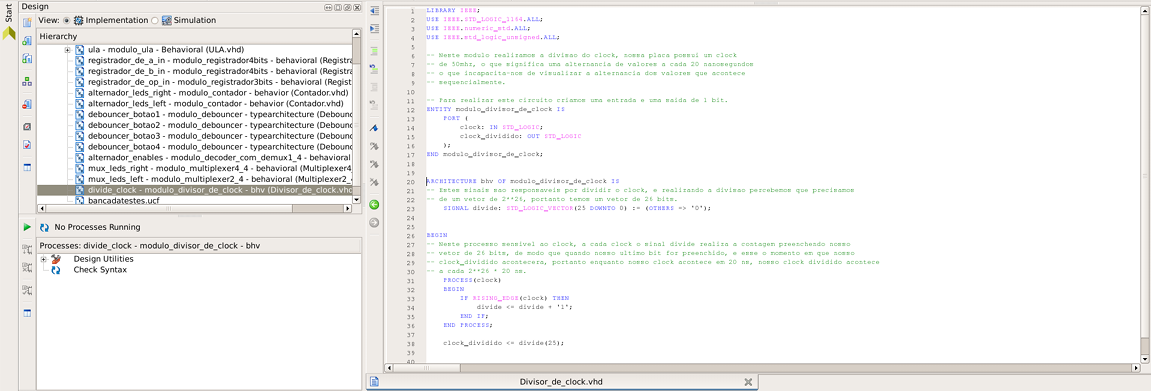
\includegraphics[width=1.1\textwidth]{codigos_divideclock.png}%
\newline\newline
O esquemático RTL e sua simulação podem ser visualizados nas imagens a seguir :
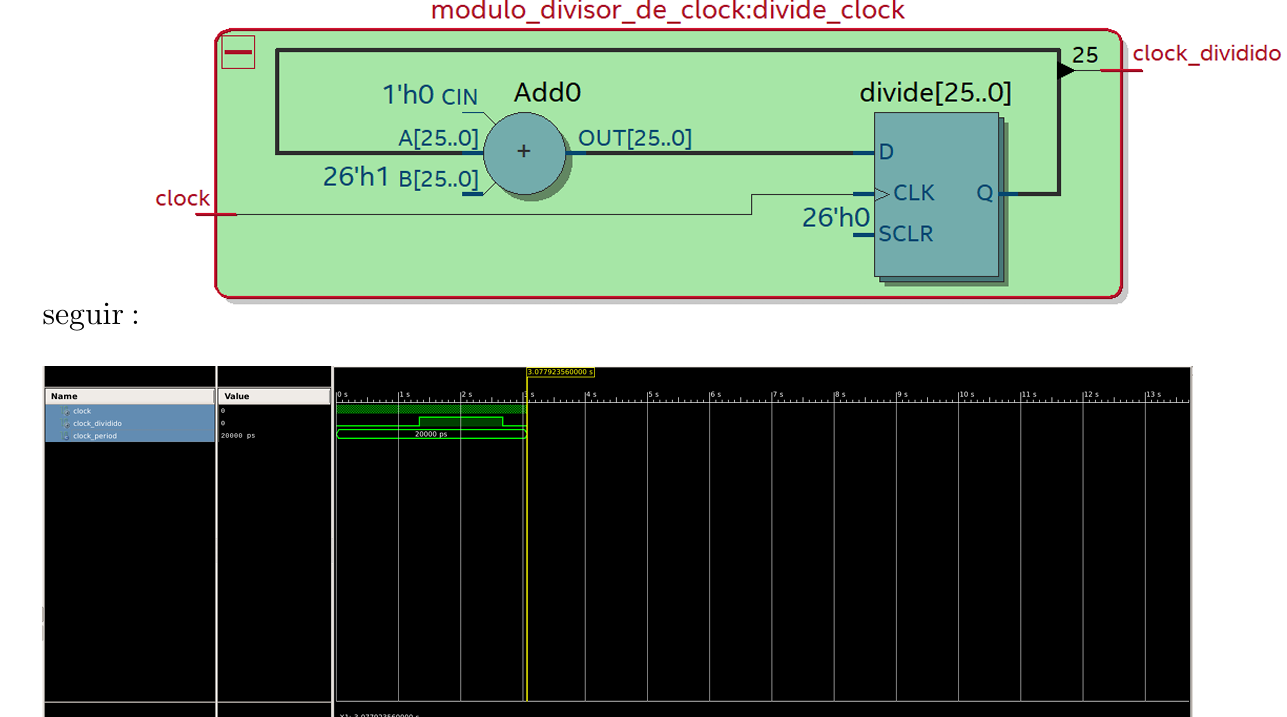
\includegraphics[width=1.1\textwidth]{RTL_divisordeclock_simulacao_clockdividido.png}%
\newline\newline


\textbf{Módulo debouncer :} 
\newline\newline
O circuito de debouncer age toda vez que apertamos ou soltamos o botão após pressionar, pois possuimos um problema de instabilidade físico nestes instantes de tempo, portanto,para resolvê-lo,  utilizaremos 3 flip flops como verificadores para saber se o sinal está estável, a cada clock um dos flip-flops recebe um delay, e quando temos o mesmo sinal nos 3 flip-flops, o sinal do botão é recebido pelo circuito sem flutuações.
\newline
O código VHDL fica da seguinte forma :

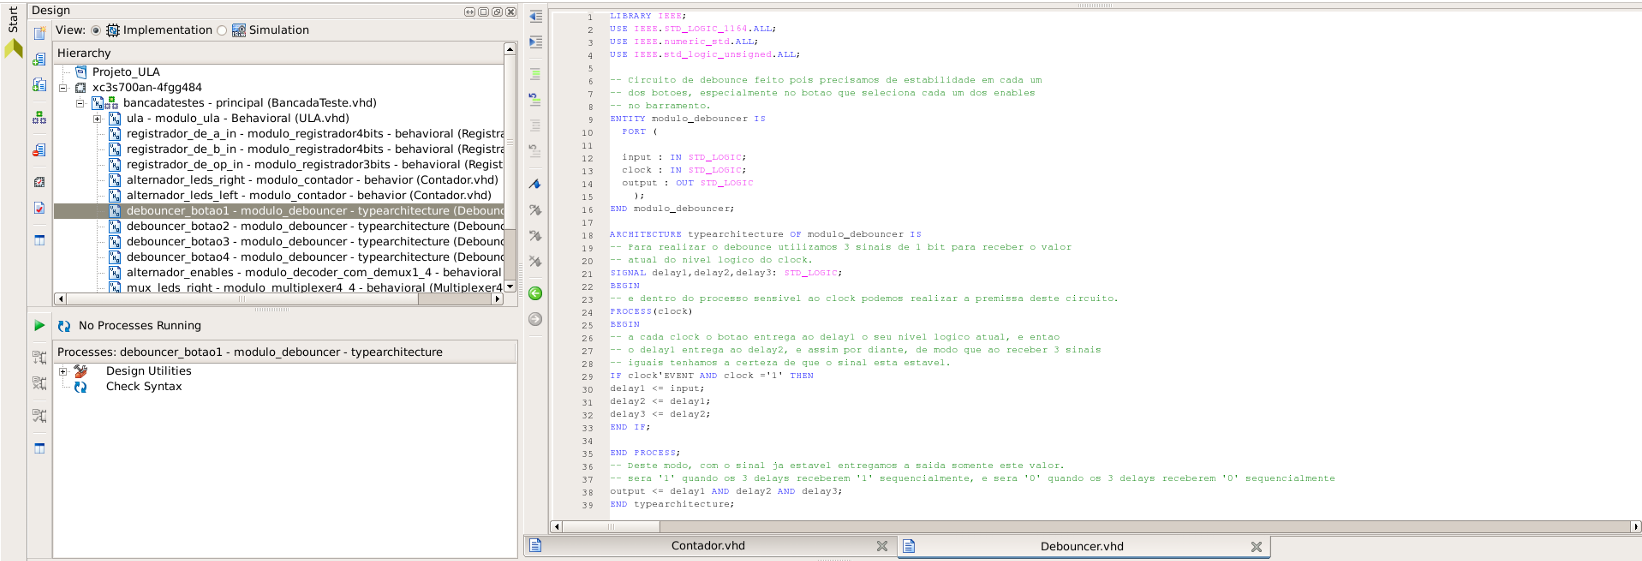
\includegraphics[width=1.1\textwidth]{codigo_debouncer.png}%
\newline
O esquemático RTL e sua simulação podem ser visualizados nas imagens a seguir :
\newline
Ex: Debouncer do botão 1 :
\newline
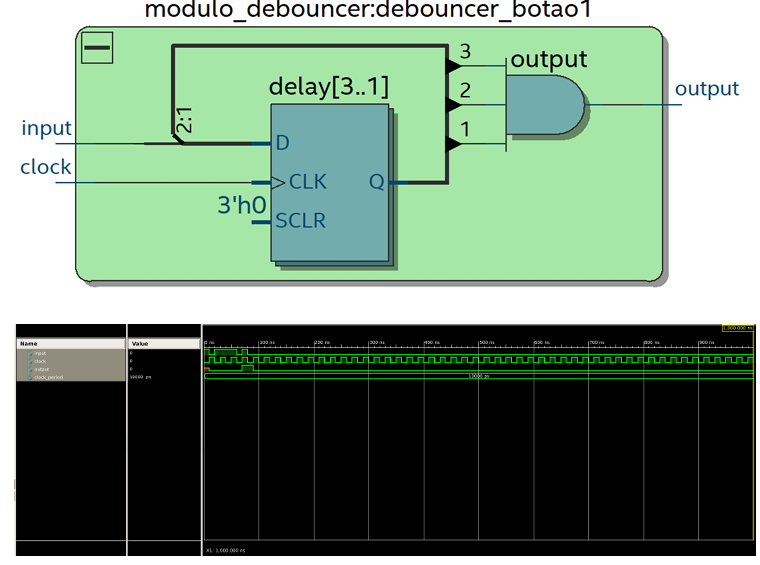
\includegraphics[width=1.1\textwidth]{RTL_botao1_debouncer_simulacao_debouncer.png}%
\newline\newline

\newpage \textbf{Módulo registrador :} 
\newline\newline
O modulo registrador de 4 e 3 bits possuem uma entrada ENABLE que foi necessaria para que pudessemos controlar o barramento, dessa forma somos capazes de utilizar uma única entrada para 3 registradores distintos, dois deles sendo este registrador de 4 bits e apenas um de 3 bits. Que são basicamente 4/3 flip-flops concatenados que registram a entrada a cada clock. 
O código VHDL fica da seguinte forma :
\newline\newline
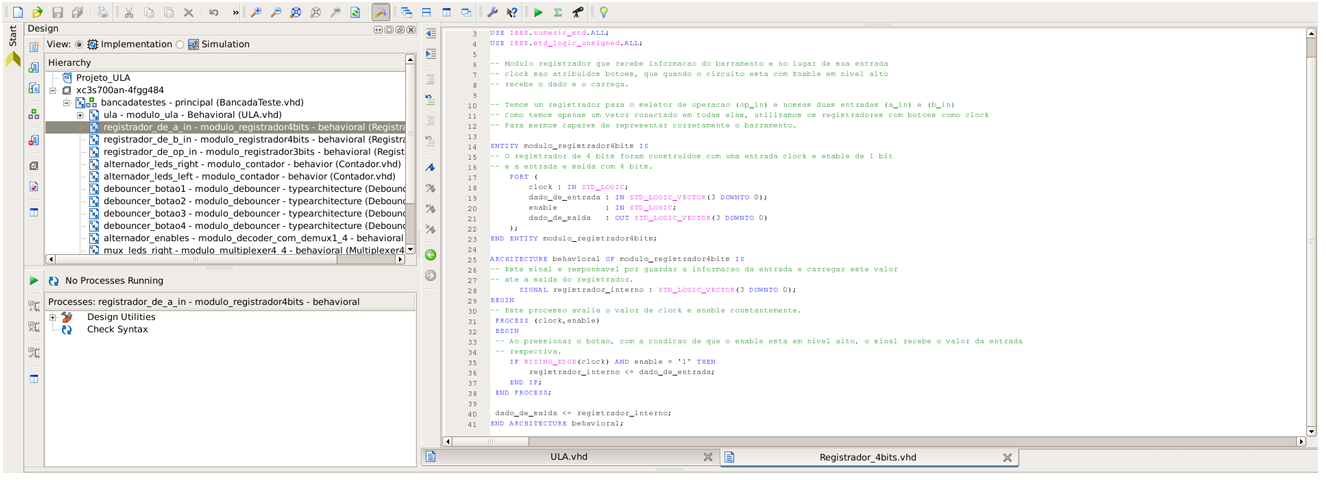
\includegraphics[width=1.1\textwidth]{codigo_registradorA.png}%
\newline
O esquemático RTL e sua simulação podem ser visualizados nas imagens a seguir :
\newline
Ex: Registrador de 4 bits :
\newline
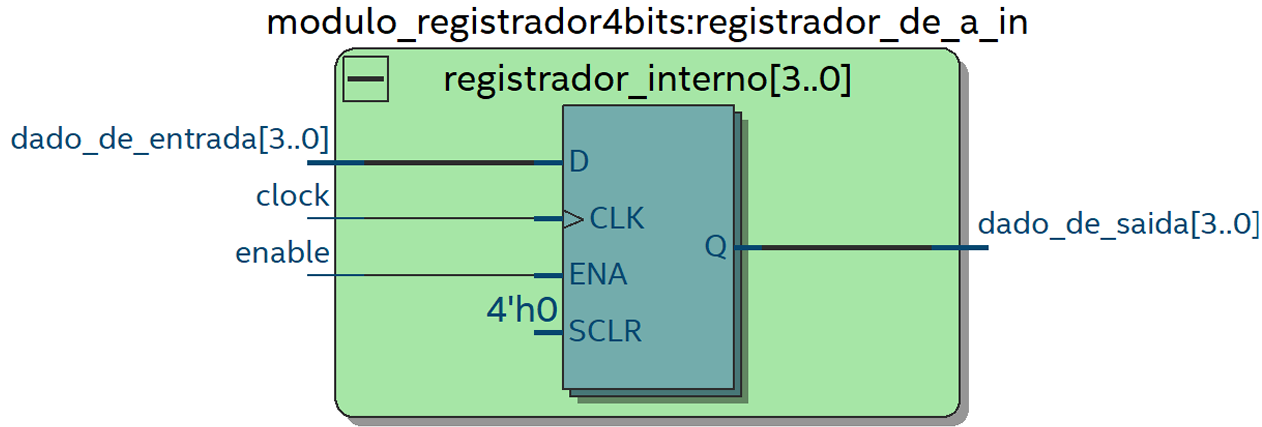
\includegraphics[width=1.1\textwidth]{RTL_registradorA.png}%
\newline\newline
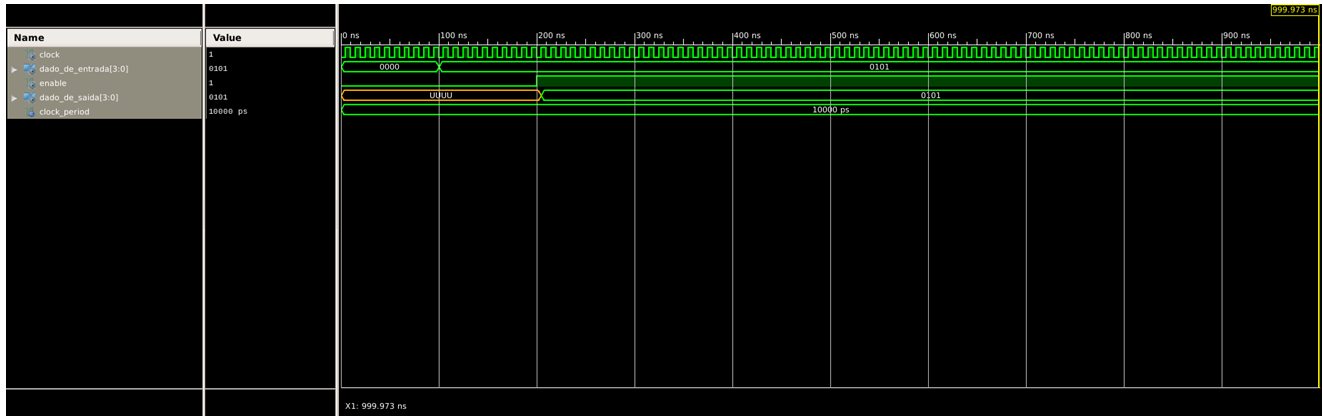
\includegraphics[width=1.1\textwidth]{simulacao_registrador.png}%
\newline


\textbf{Módulo Contador :} 
\newline\newline
Foi projetado um contador simples, pois precisávamos alternar nossa sáida junto ao clock de maneira controlada, portanto temos apenas um flip-flop que realimenta sua entrada com o valor anterior, obtendo então : 
\newline\newline
$temp = temp + 1$ obtendo assim um contador que varia de 1 até 4, pois temos apenas 2 flip-flops concatenados.
\newline\newline
O código VHDL fica da seguinte forma :
\newline\newline
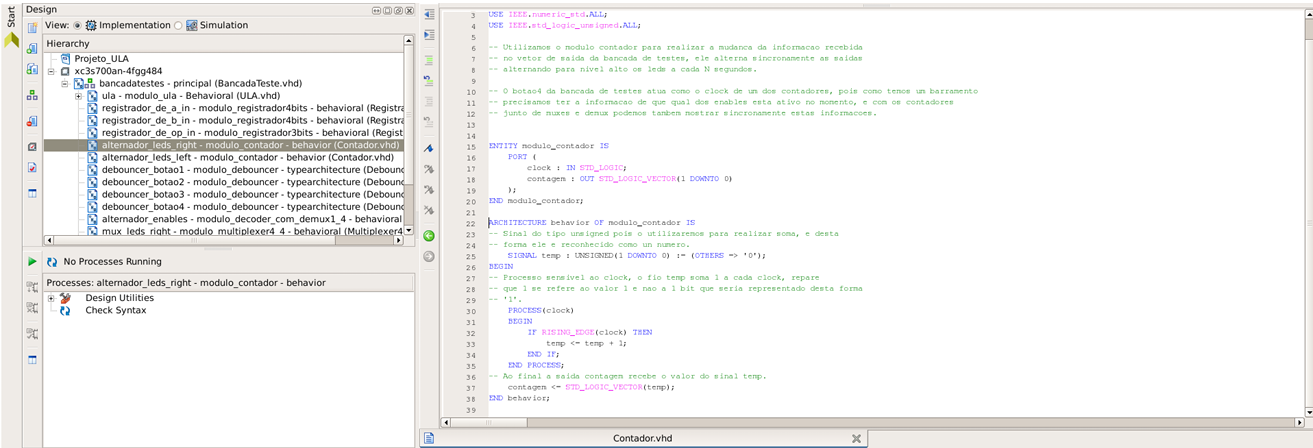
\includegraphics[width=1.1\textwidth]{codigo_contador.png}%
\newline
O esquemático RTL e sua simulação podem ser visualizados nas imagens a seguir :
\newline
\newpage Ex: Contador que altera LEDS da direita :
\newline
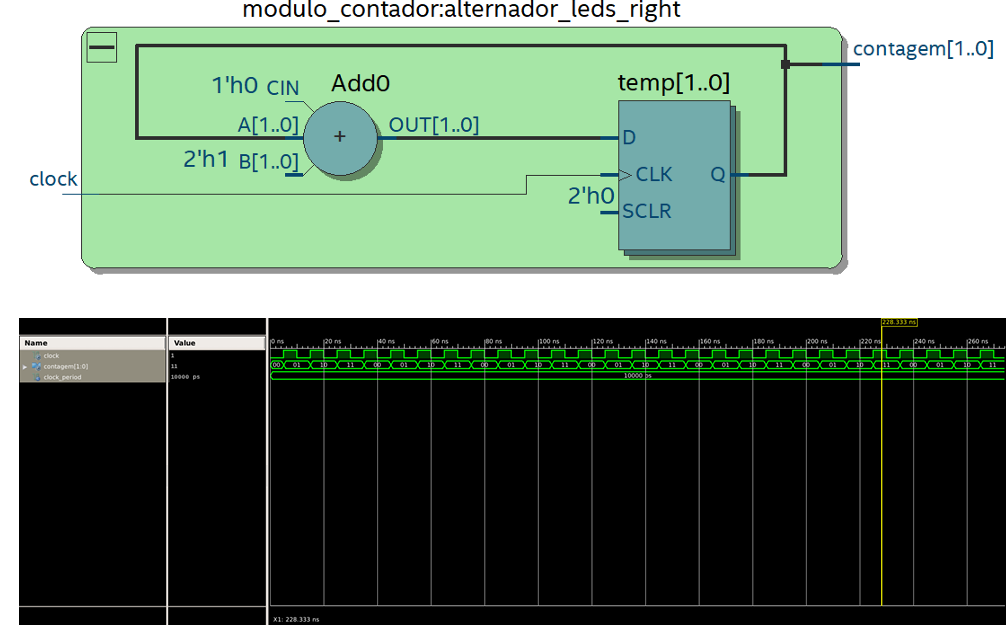
\includegraphics[width=1.1\textwidth]{RTL_contadorLEDSdireita_simulacao_contador.png}%
\newline


\textbf{Módulo decodificador :} 
\newline\newline
Como decodificador utilizamos uma demux com sua entrada de 1 bit alimentada em nivel alto, ela é responsável por habilitar cada um dos Enables dos registradores a cada clock ( que nesse caso seria o nosso botão 4 fazendo o papel de clock), desse modo temos que : 
\newline
O código VHDL fica da seguinte forma :
\newline\newline
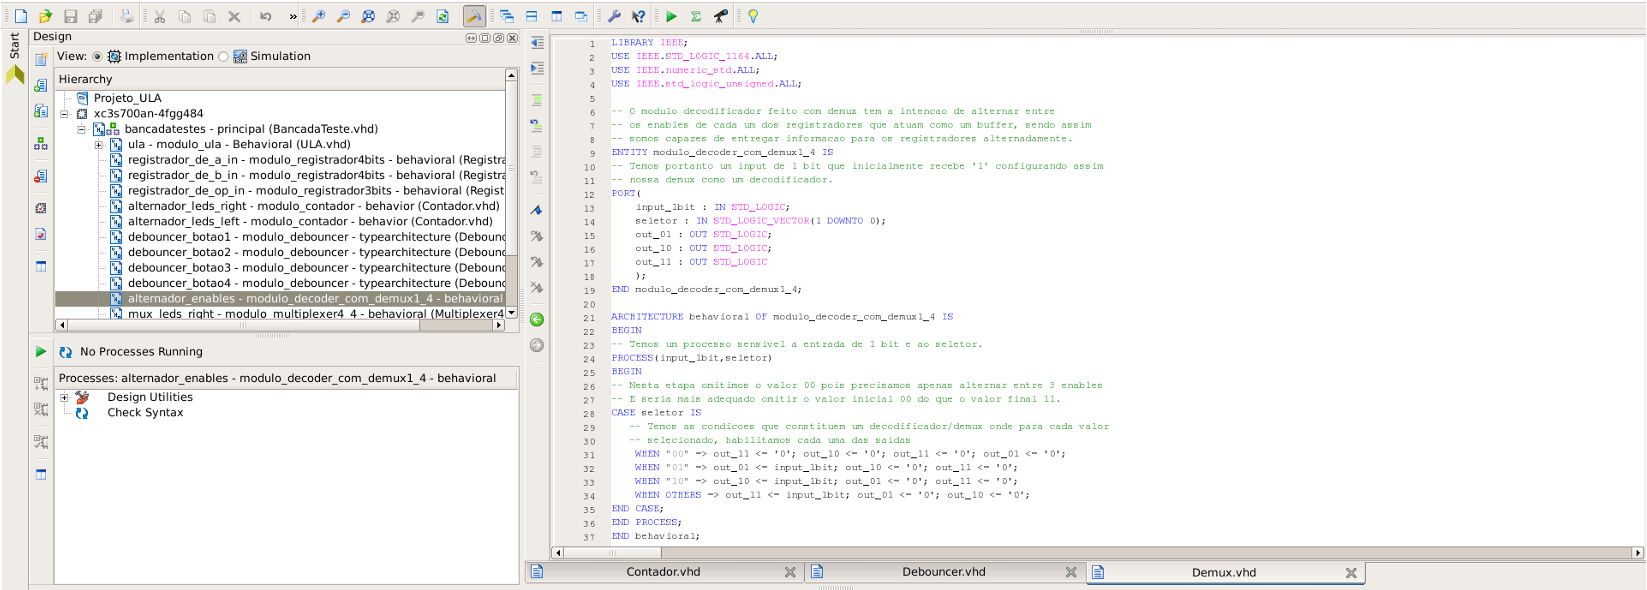
\includegraphics[width=1.1\textwidth]{codigo_demuxdecoder.png}%
\newline
 Ex: Decoder feito com Demux :
\newline\newline
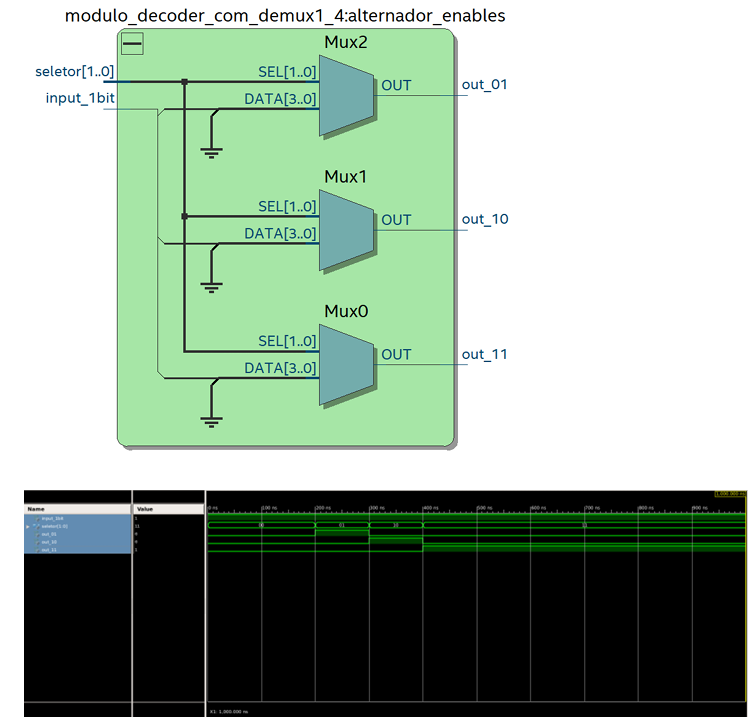
\includegraphics[width=1.1\textwidth]{RTL_demux_decoder_simulacao_decoderDEMUX.png}%
\newline


\textbf{Módulo Mux :} 
\newline\newline
Utilizamos dois módulos distintos de Mux, a diferença entre elas são somente a quantidade de entradas, sendo uma mux de quatro entradas de 4 bits e a outra com duas entradas de 4 bits, este módulo foi essencial para que pudéssemos distribuir entre os LEDS do resultado onde cada flag,entrada,resultado e operação apareceria sequencialmente.
O código VHDL da mux de quatro entradas de 4 bits fica da seguinte forma :
\newline\newline
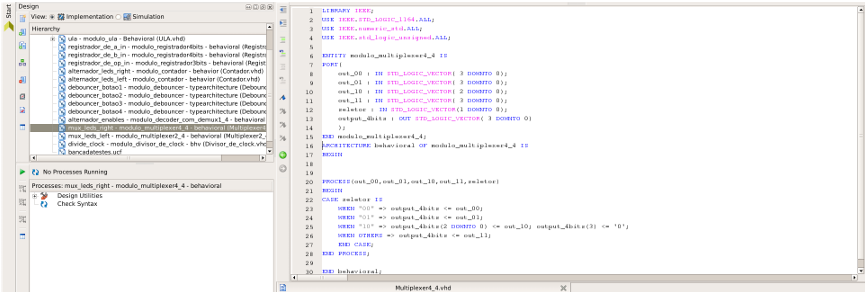
\includegraphics[width=1.1\textwidth]{codigo_multiplexer44.png}%
\newline
O esquemático RTL e sua simulação podem ser visualizados nas imagens a seguir :
\newline
Ex: Mux de duas entradas de 4 bits(obs: uma das entradas foram aproveitados apenas 2 bits, pois se refere ao Enable selecionado no momento, que vem do contador controlado pelo botão 4 :
\newline
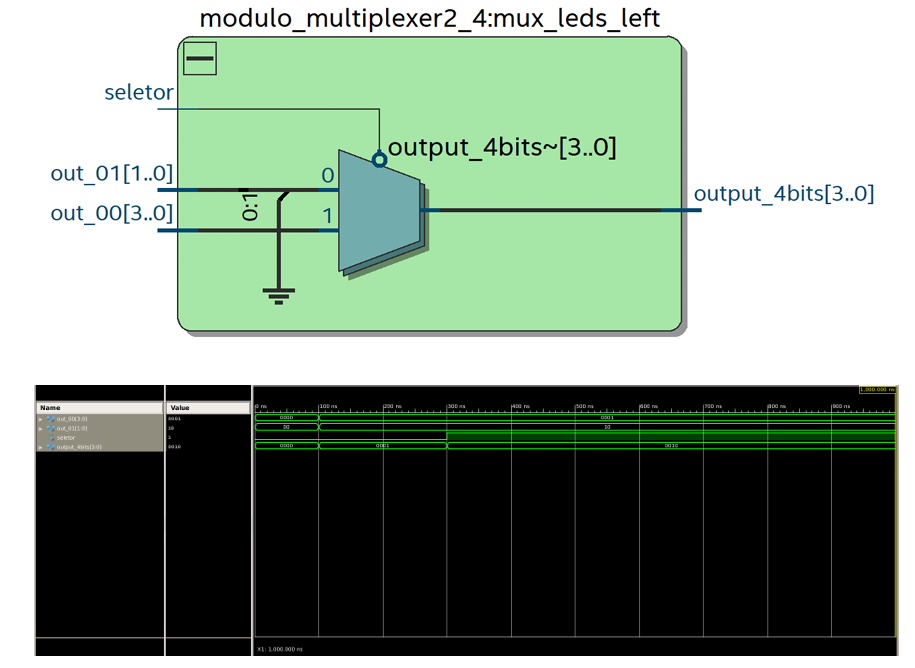
\includegraphics[width=1.1\textwidth]{RTL_mux24_simulacao_multiplexador24.png}%
\newline


\textbf{Módulos de operações aritiméticas :} 
\newline\newline
Para as operações aritiméticas temos as seguintes : Soma e subtração, para realizar cada um deles projetamos um somador de 4 bits e realizamos o complemento de 2 reaproveitando o mesmo módulo somador habilitando usa entrada $carry in$ e negando o sinal da entrada B, sendo assim obtemos além do somador, também um subtrator. 
O código VHDL fica da seguinte forma :
\newline\newline
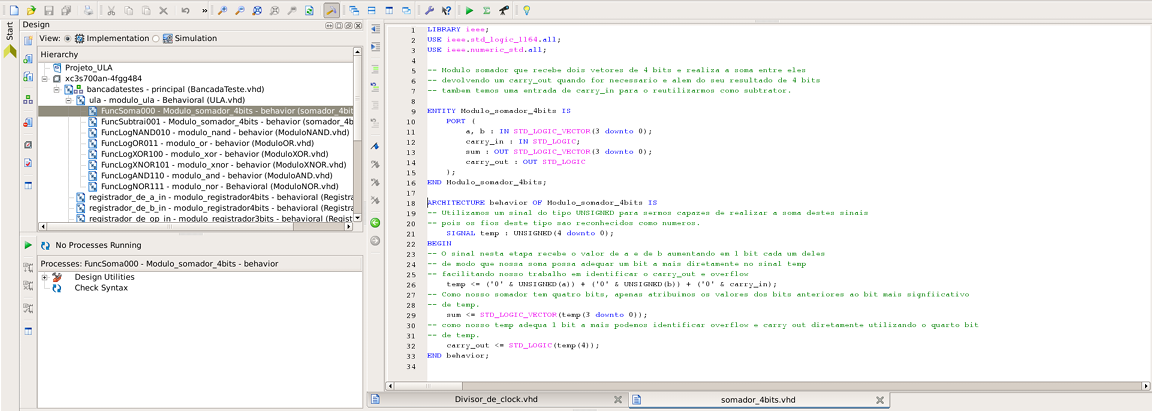
\includegraphics[width=1.1\textwidth]{codigo_somador.png}
\newline
O esquemático RTL e sua simulação podem ser visualizados nas imagens a seguir :
\newline
Ex: Mux de duas entradas de 4 bits(obs: uma das entradas foram aproveitados apenas 2 bits, pois se refere ao Enable selecionado no momento, que vem do contador controlado pelo botão 4 :
\newline
\newline
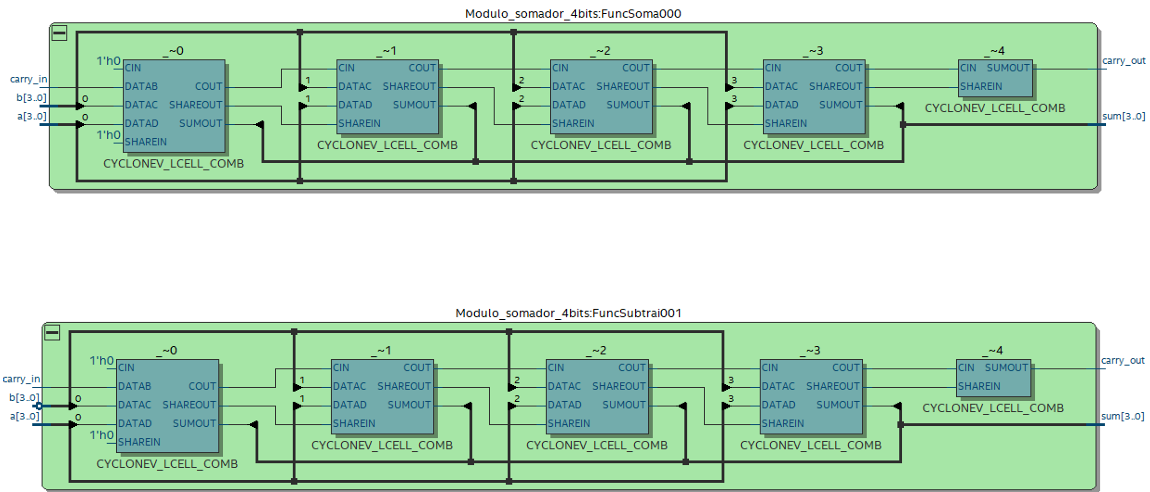
\includegraphics[width=1.1\textwidth]{RTL_modulo_somador_subtrator.png}%
\newline\newline


\newpage \textbf{Módulo de operações lógicas :} 
\newline\newline
Projetando as operações lógicas utilizamos diretamente a praticidade de se utilizar a linguagem VHDL, portanto conseguimos diretamente nossa operação apenas indicando se AND, NAND, OR, NOR, XOR, XNOR para a linguagem, logo temos : 
Por exemplo o codigo VHDL da porta lógica AND :
\newline\newline
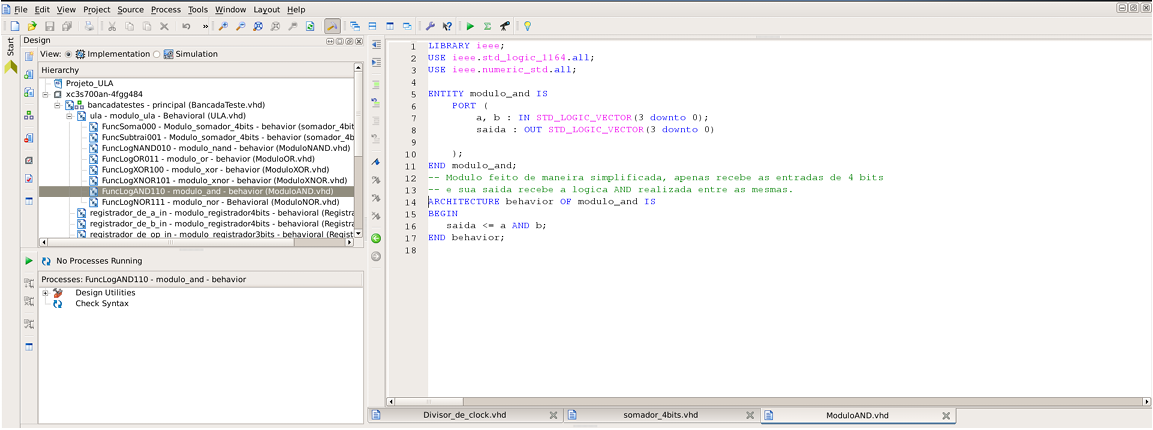
\includegraphics[width=1.1\textwidth]{codigo_andgate.png}%
\newline
O esquemático RTL e sua simulação podem ser visualizados nas imagens a seguir :
\newline
Ex: Operação lógica XNOR : 
\newline
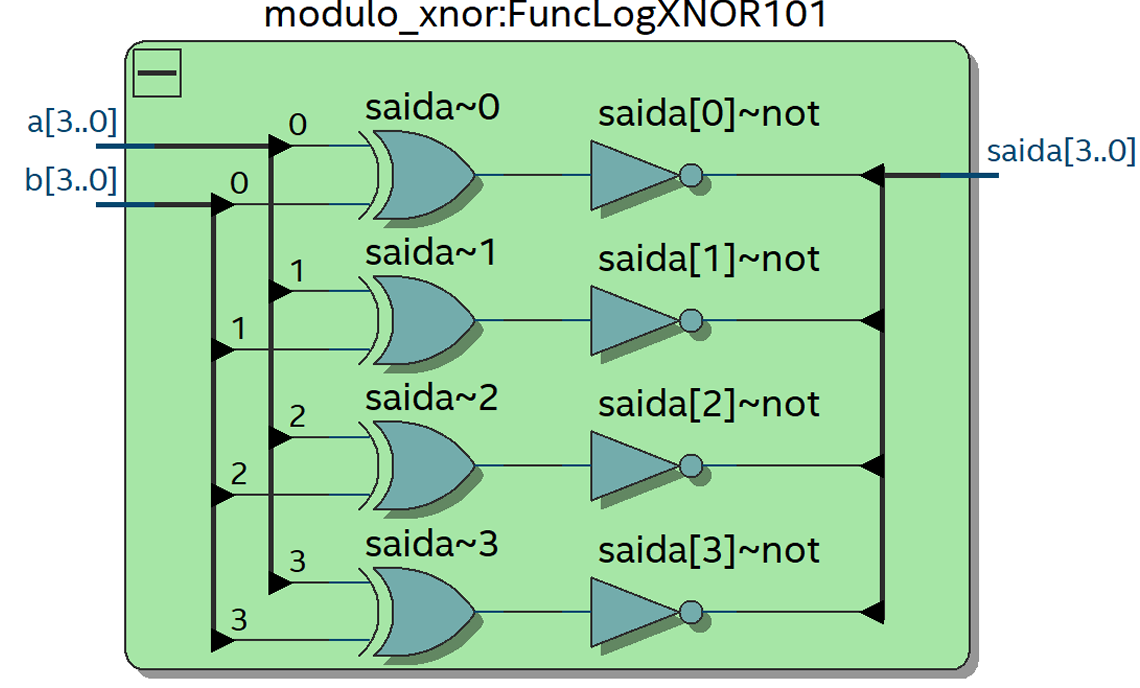
\includegraphics[width=1.1\textwidth]{RTL_xnor.png}%
\newline\newline


\textbf{Módulo ULA :} 
\newline\newline
O projeto do módulo ULA consistiu em : 
\newline\newline
\begin{itemize}
    \item Projetar módulos de funções lógicas e aritiméticas.
    \item Utilizar o código base da ULA somente como bancada, ou seja, no seu código consta apenas seus componentes, o mapeamento, os sinais(fios) e a configuração em que cada operação será realizada.  
\newline\newline
    O código VHDL da ULA:
\newline\newline
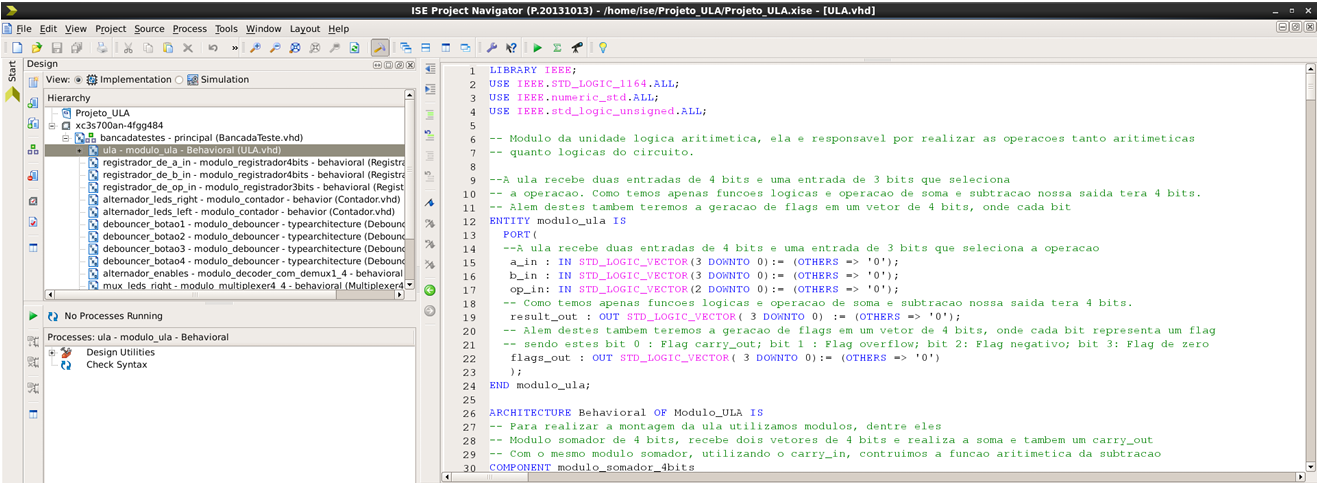
\includegraphics[width=1.1\textwidth]{Codigo_ULA.png}
\newline
    Declaração de componentes da ULA:
\newline\newline
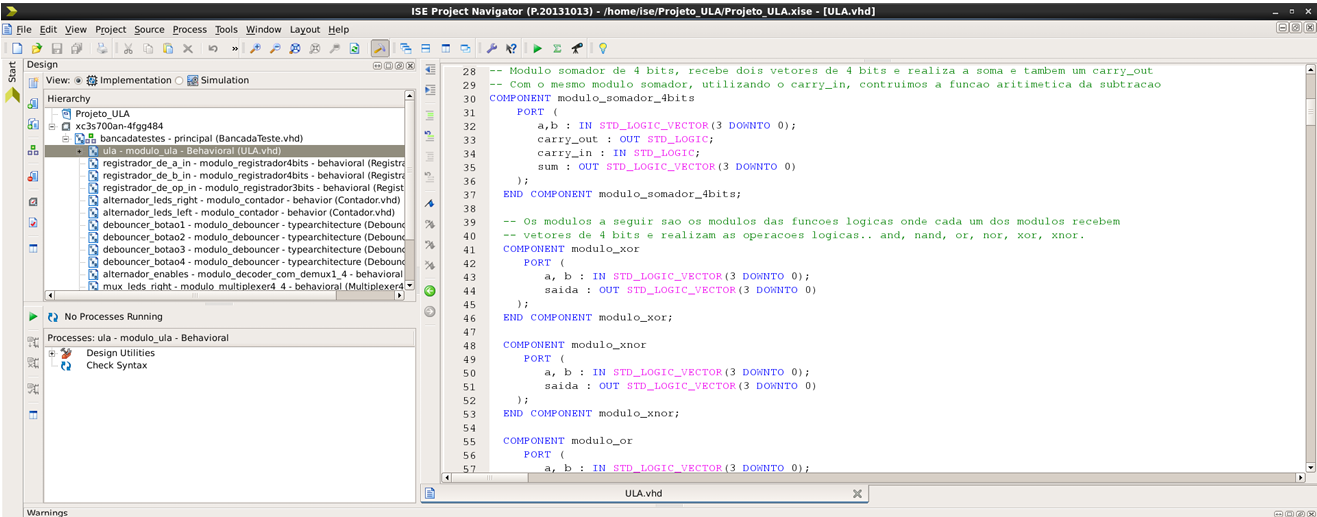
\includegraphics[width=1.1\textwidth]{ULA_comp_cod.png}
\newline
    Mapeamento dos componentes da ULA :
\newline\newline
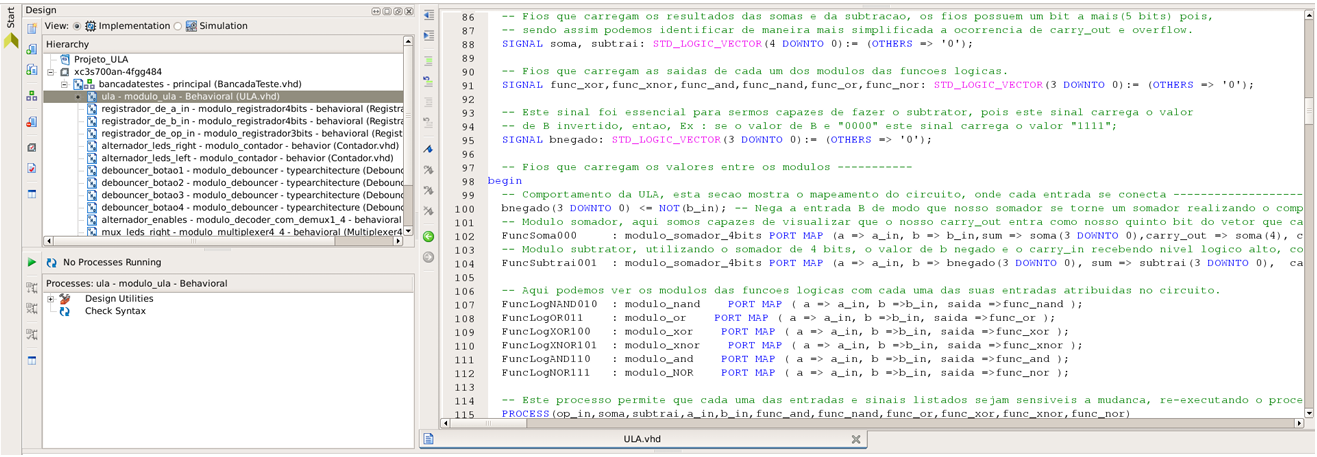
\includegraphics[width=1.1\textwidth]{ULA_comp.png}
\newline
    \item As operações seguiriam o padrão : Primeiro as operações aritiméticas, e após as operações lógicas, portanto temos : Ex : 000 SOMA ; 001 SUBTRAÇÃO ; 010 AND ; 011 NAND ; 100 OR ; 101 NOR...
    \item As flags das operações aritiméticas são bit/flag : (0)ZERO, (1)NEGATIVO, (2)CARRY OUT E (3)OVERFLOW.
    \newline\newline
    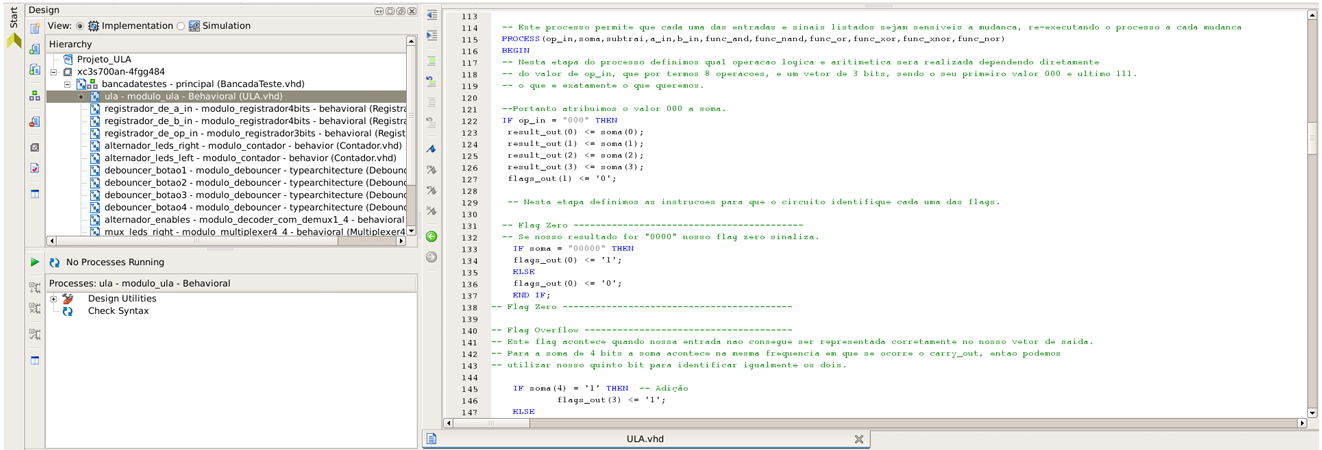
\includegraphics[width=1.1\textwidth]{flagss.png}
    \newline
    \item As flags das operações lógicas são bit/flag : (2 e 3 em '0')NENHUMA PORTAS LÓGICAS ATIVA ; (2 em '1')PELO MENOS UMA PORTAS LÓGICAS ATIVA ; (3 em '1')NUMERO IGUAL DE PORTAS LÓGICAS ATIVAS ; (2 e 3 em '1')TODAS ATIVAS.
    \newline\newline
    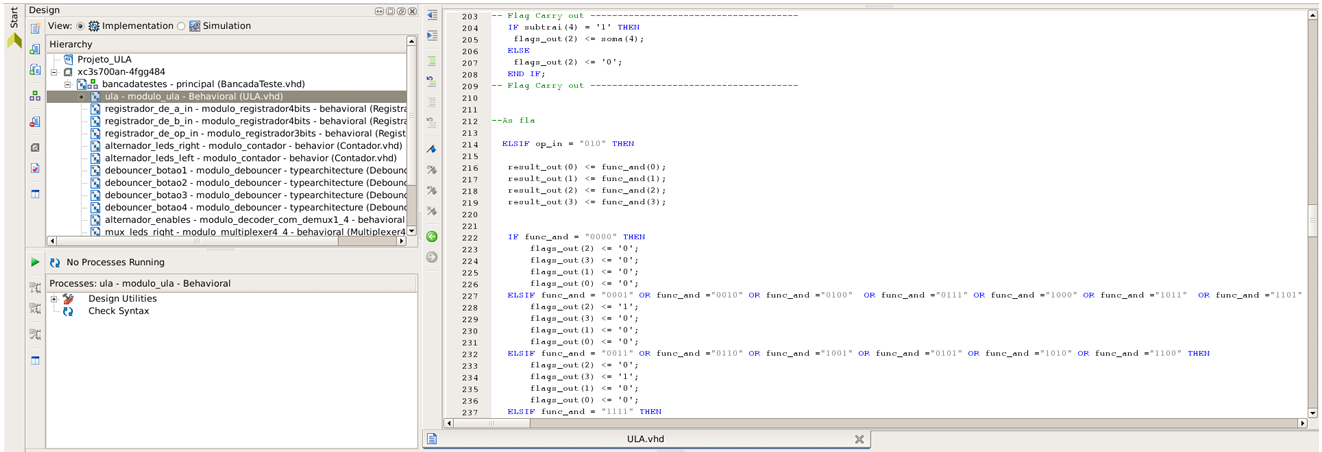
\includegraphics[width=1.1\textwidth]{flags.png}
    \newline
\end{itemize}
O esquemático RTL e sua simulação podem ser visualizados nas imagens a seguir :
\newline
\newline
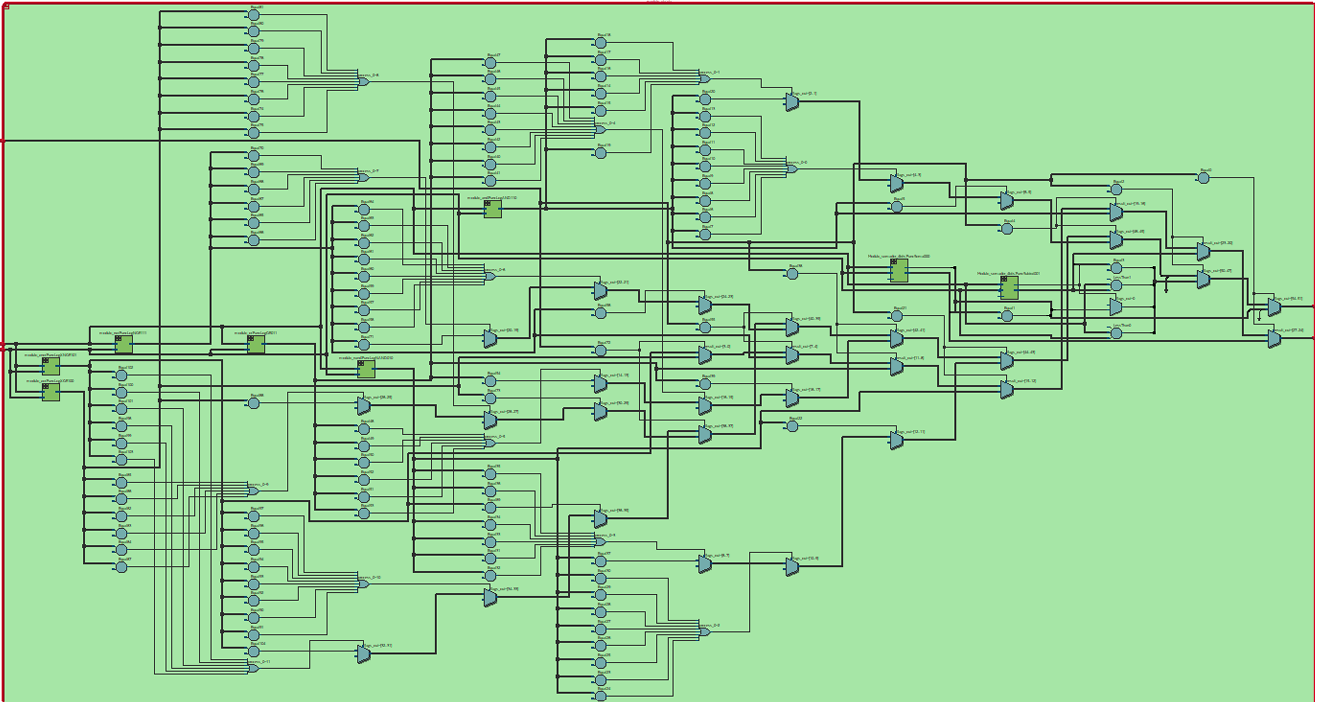
\includegraphics[width=1.1\textwidth]{Simulacao_RTL.png}%
\newline\newline
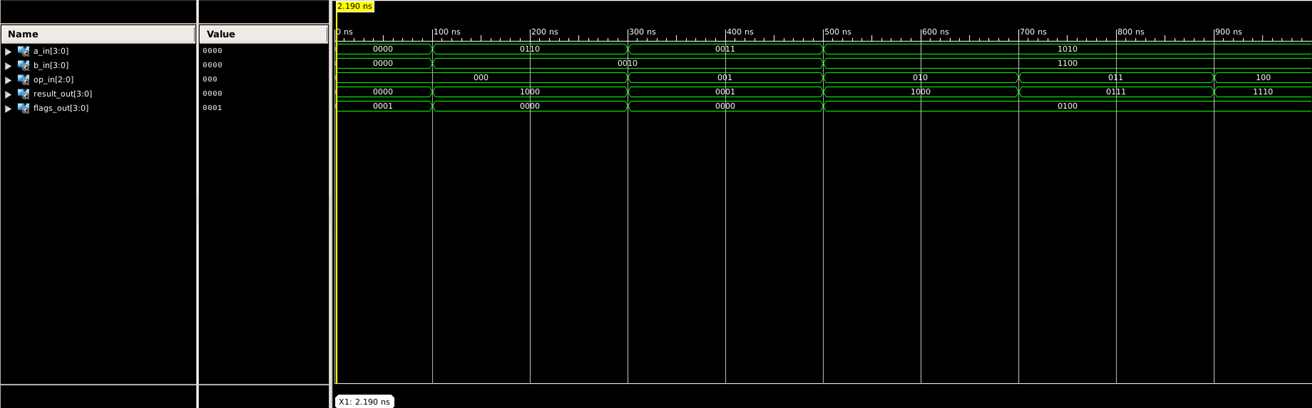
\includegraphics[width=1.1\textwidth]{Simulacao_ULA.png}\\
\textbf{Obs: As simulações dos módulos somador, subtrator e funções lógicas constam dentro da simulação da ULA, portanto decidimos simplificar apenas mostrando o da ULA.}
\newline
\newline
\textbf{Ao fim teremos esta configuração entre a bancada de testes e a ULA, a seguir existe a relação entre fonte dos dados e saída dos mesmos.}
\newline
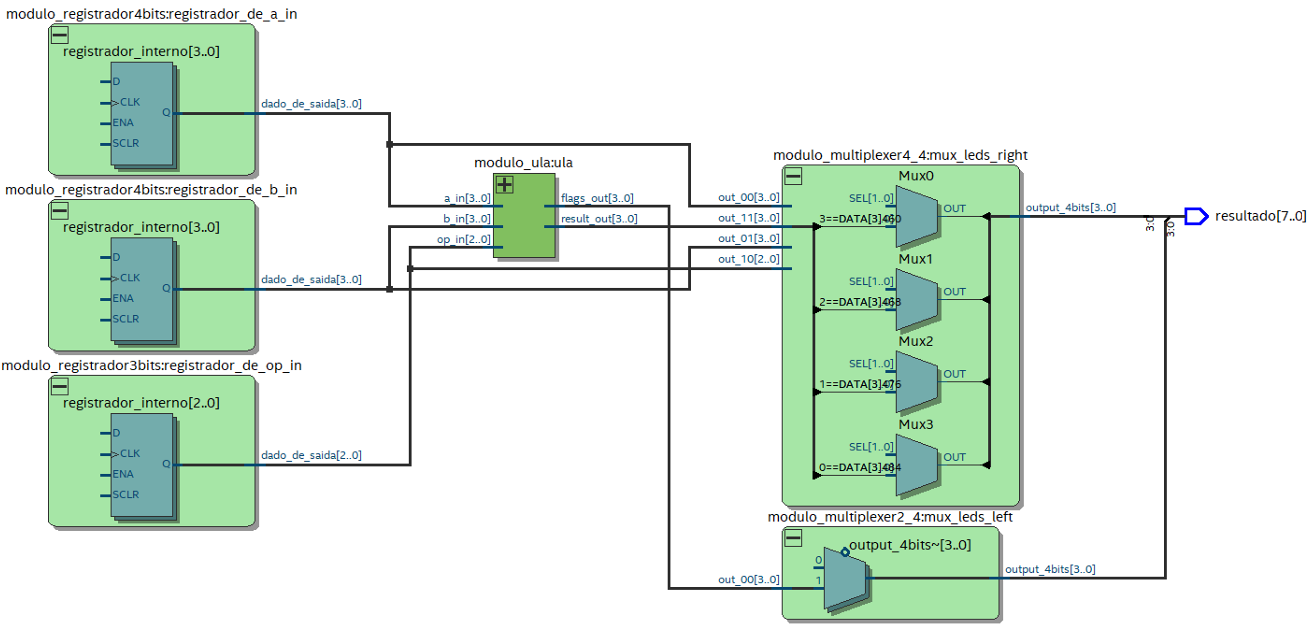
\includegraphics[width=1.1\textwidth]{Config_Bancada_ULA.png}%
\newline\newline


\textbf{Bancada de testes : }
\newline\newline
A bancada de testes foi feita exatamente como a ULA, declaração de componentes, e após feita configuração dos sinais e mapeamento apenas tivemos o trabalho de delegar quais bits da saída Resultado de 8 bits seria alimentado.
A configuração final ficou da seguinte forma : 
\begin{itemize}
    \item 4 Switches é representado por uma entrada vetorial de 4 bits e indica o valor das  nossas entradas em geral.
    \item Botões 1,2,3,4 agem como clock em nosso circuito, de modo que ao pressionar Botão 1 ou Botão 2 ou Botão 3 que indicam respectivamente os clocks do Registrador A, Registrador B e Registrador de Operação, se o Enable correspondente estiver ativo, a entrada é registrada. E o nosso botão 4 é responsável por alternar a alimentação dos enables dos registradores de A, B e Operação.
    \item 8 LEDS é representado por uma entrada vetorial de 8 bits e indica o valor das nossas saídas e flags Resultado. Os 4 leds mais à \textbf{esquerda} indicam : Flags e enable ativo, sendo que os flags utilizam os 4 leds e o enable apenas 2 ( contando da direita para a esquerda). Os 4 leds mais à \textbf{direita} indicam : Entrada A, Entrada B, Operação e Resultado, respeitam esta sequência, com a observação de que a operação utiliza apenas 3/4 leds.
    \item Clock é utilizado tanto como indicador para o debounce, como também para a alternância junto aos contadores e muxes, considerando o clock da placa e o dividido, permitindo que alterne sequencialmente.  
\end{itemize}
O código VHDL da Bancada de testes:
\newline\newline
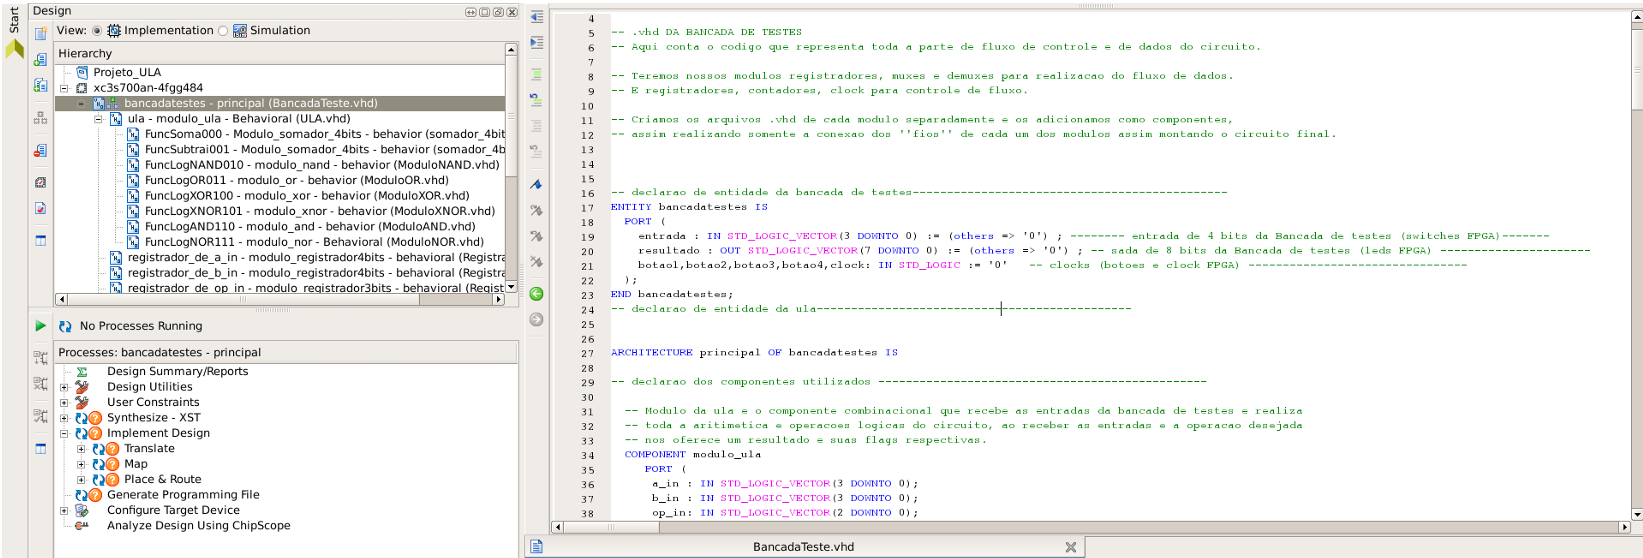
\includegraphics[width=1.1\textwidth]{Codigo_Bancada.png}
\newline
\newpage O código do mapeamento da Bancada de testes:
\newline\newline
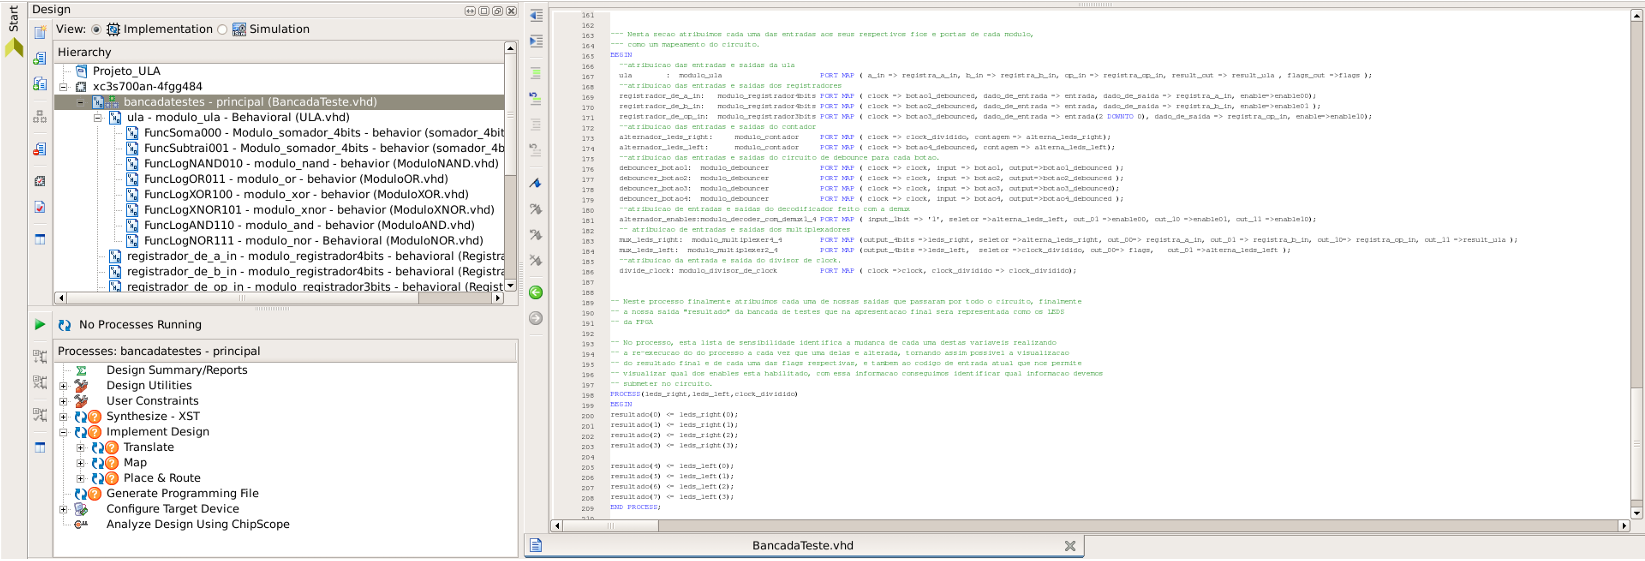
\includegraphics[width=1.1\textwidth]{Codigo_Map.png}
\newline
O código VHDL da arquitetura da bancada de testes:
\newline\newline
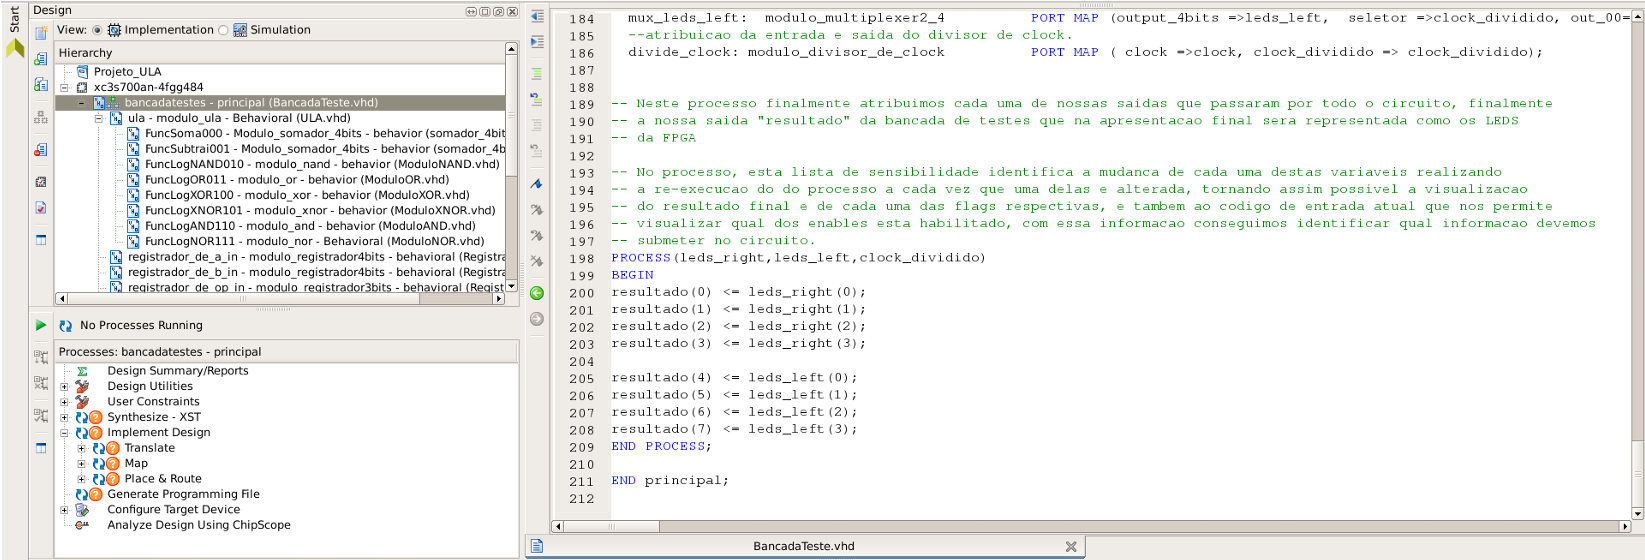
\includegraphics[width=1.1\textwidth]{Codigo_Arquitetura.png}
\newline
O código dos sinais(fios) da bancada de teste:
\newline\newline
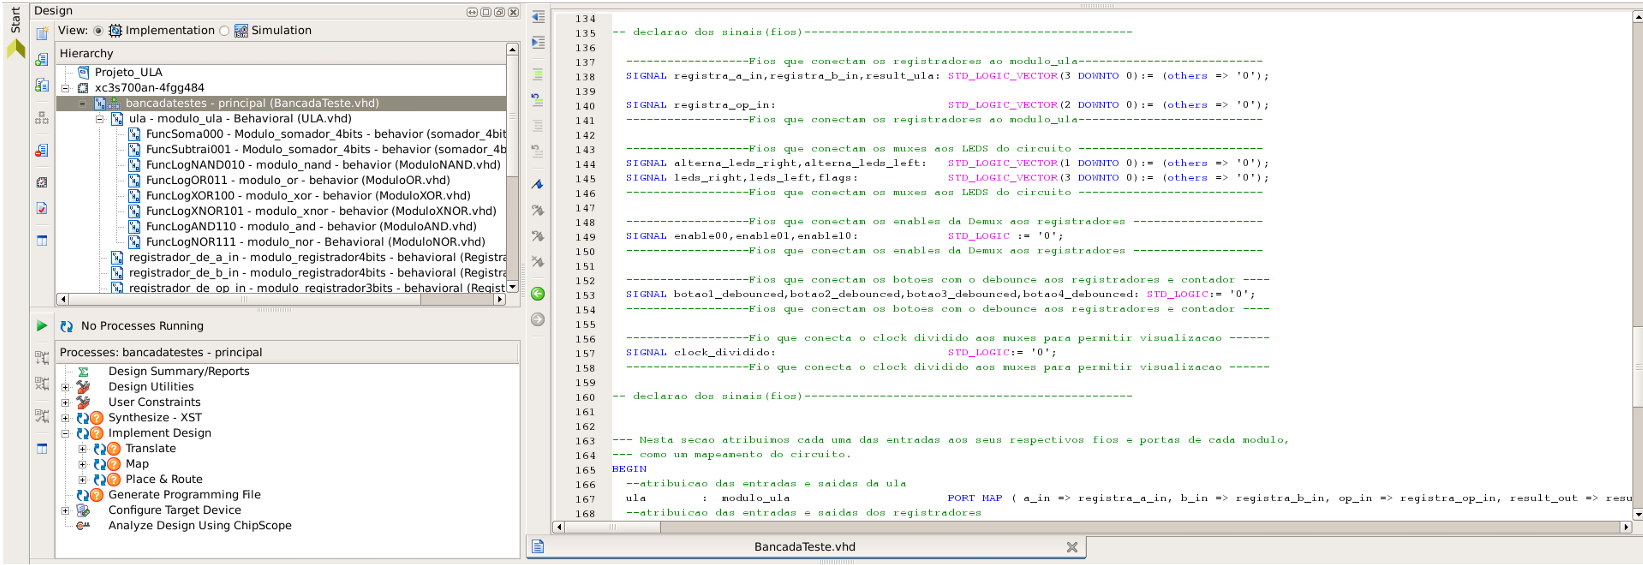
\includegraphics[width=1.1\textwidth]{Codigo_Sinais.png}
\newline
\newpage O esquemático RTL e sua simulação podem ser visualizados nas imagens a seguir :
\newline
\newline
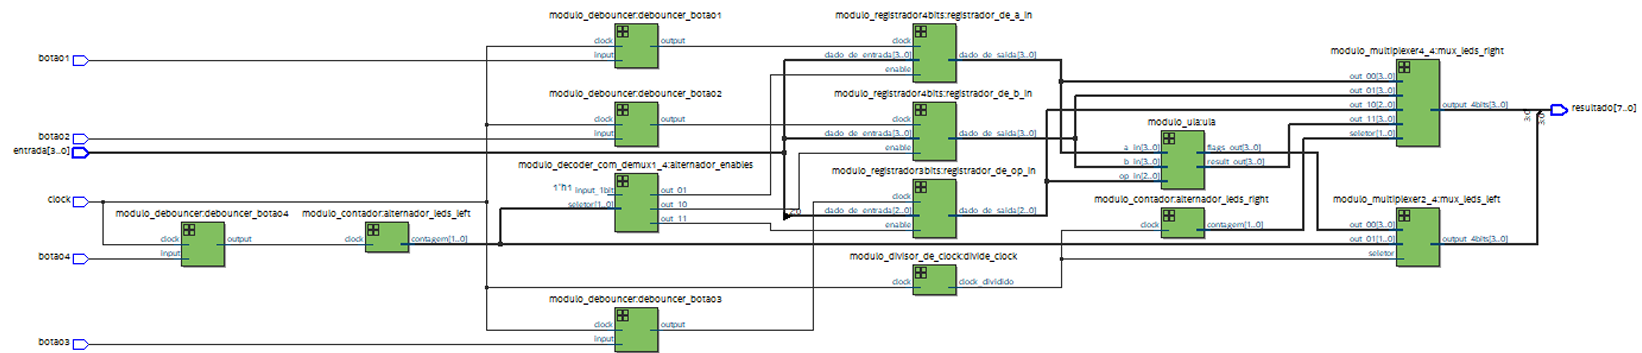
\includegraphics[width=1.1\textwidth]{Esquematico_RTL.png}%
\newline\newline
Simulação bancada de testes : 
\newline\newline
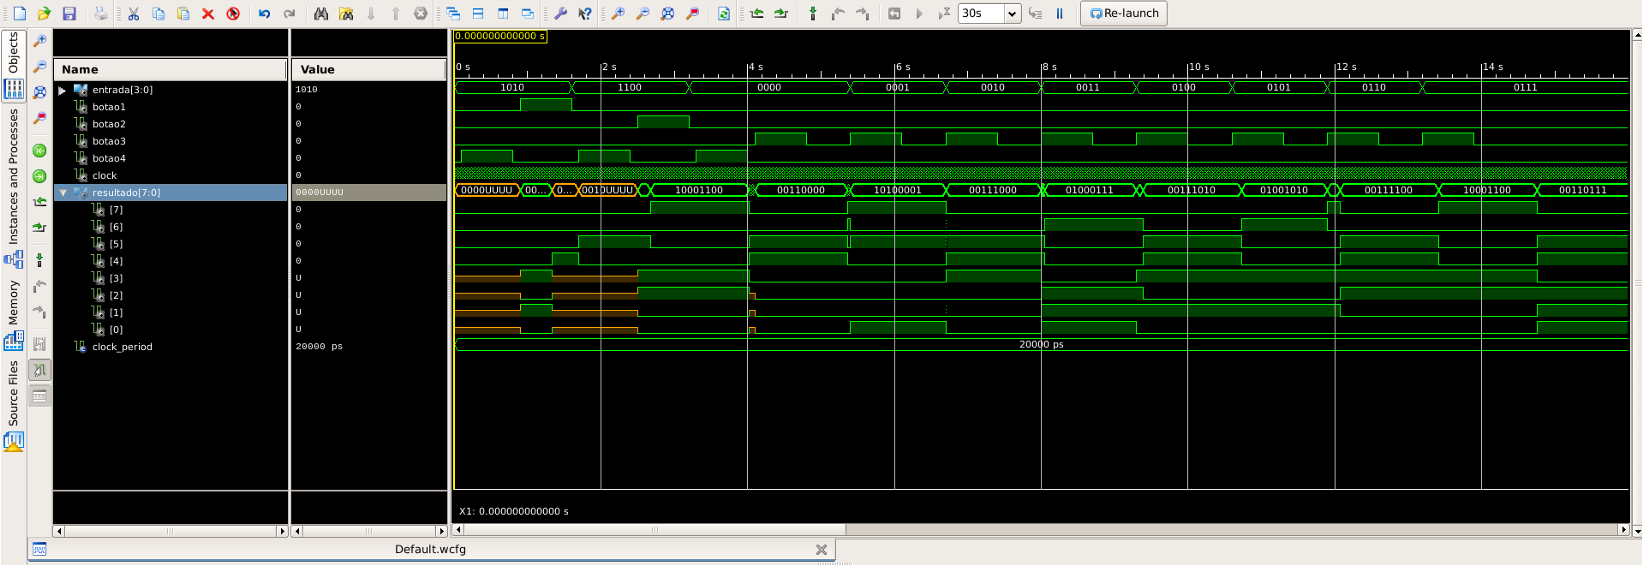
\includegraphics[width=1.1\textwidth]{Simulacao_Bancada_de_Testes.png}%
\newline\newline
Simulação das Flags Lógicas de algumas portas lógicas : 
\newline\newline
Porta AND :
\newline\newline
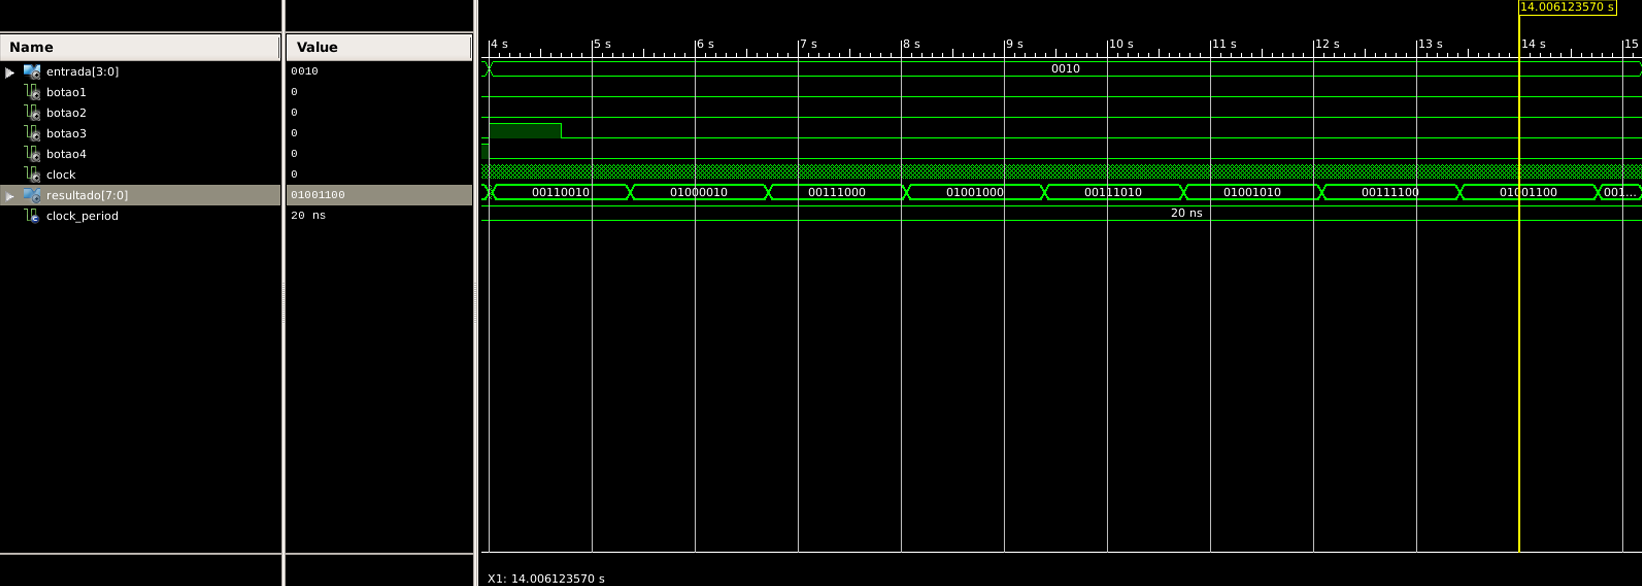
\includegraphics[width=1.1\textwidth]{Porta_AND.png}%
\newline\newline
 Porta OR:
\newline\newline
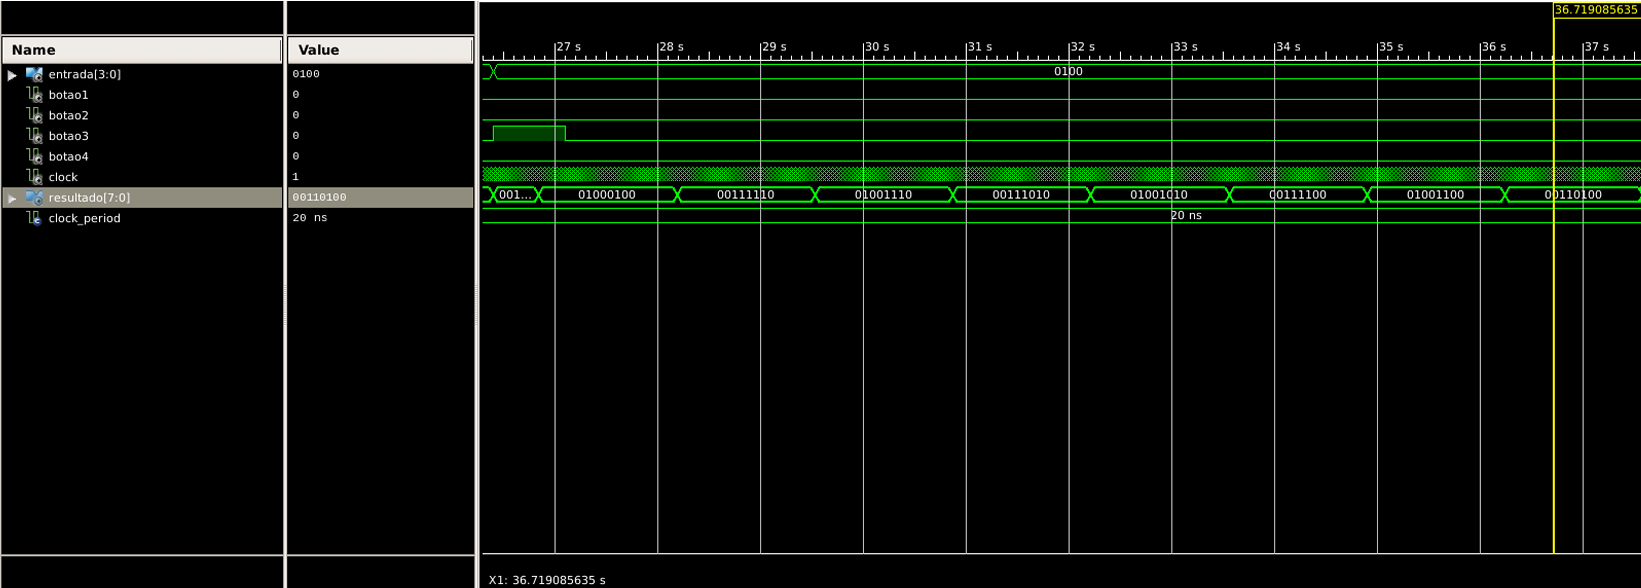
\includegraphics[width=1.1\textwidth]{Porta_OR.png}%
\newline\newline
Porta XOR:
\newline\newline
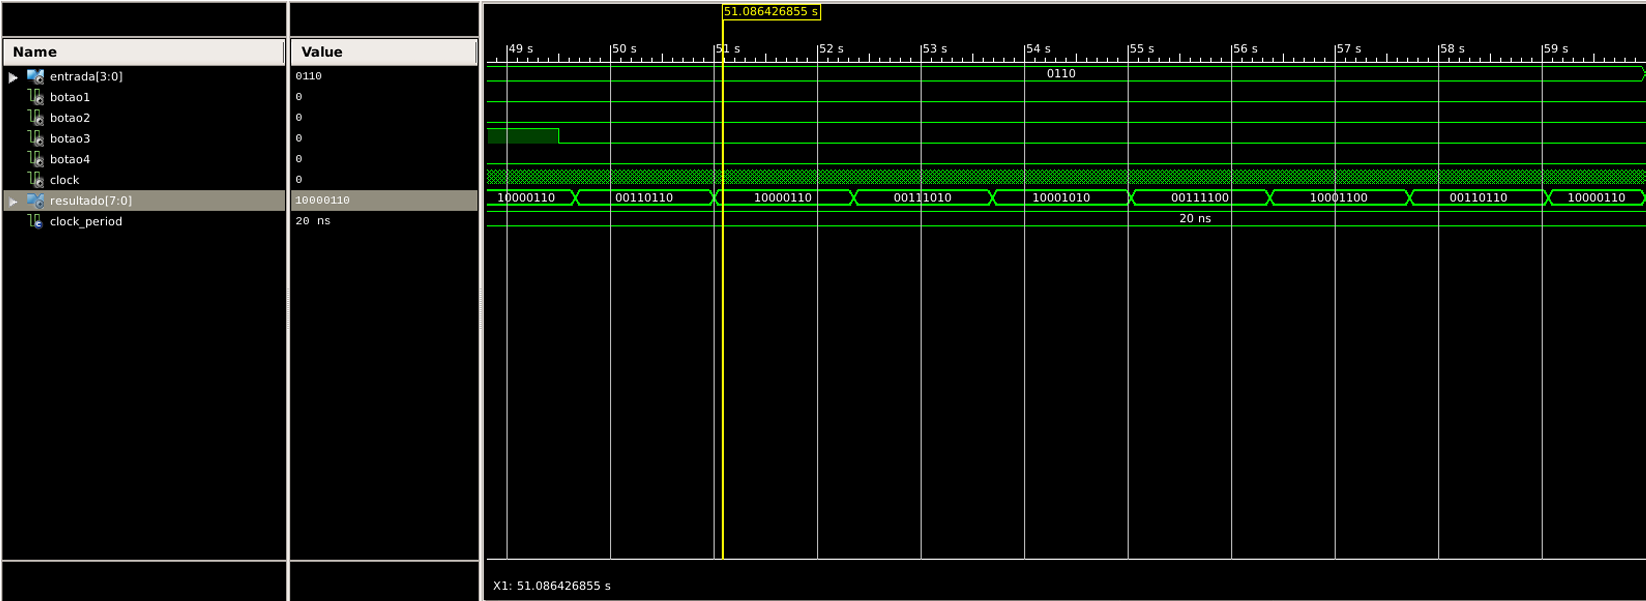
\includegraphics[width=1.1\textwidth]{Porta_XOR.png}%
\newline\newline
\textbf{Obs : Como nosso clock dividido possui um tempo de 1,34s precisamos de 4 ciclos para a alternagem total dos leds mais à direita (Entrada A, Entrada B, Entrada Operação, Resultado) enquanto à esquerda em apenas 2 ciclos conseguimos identificar o Enable atual ativo e as Flags.}  

        \chapter{Conclusão}
        \section{Observações:}
        \begin{itemize}
            \item No inicio não estava muito claro que deveríamos utilizar a ULA como módulo e não como a bancada de testes, no andamento do trabalho, vimos que ao usarmos a ULA como módulo, além de organizar o projeto, existe uma permissibilidade de reutilizar o módulo ULA, e isto era exatamente o que buscávamos.
            \item Organizar o projeto em módulos separados possibilitou a fácil manutenção e visualização em nível alto. 
            \item Fez-se claro inteligível como o PORT MAP, SIGNAL, COMPONENTS, etc funcionam na linguagem VHDL, o que facilitou a compreensão do projeto ao visualizarmos ele como um mapeamento de fios que conectam as entradas de cada módulo do circuito entre si. 
        \end{itemize}

        
    \chapter{Referências Bibliográficas}
        \section{Como usar o VHDL:}
        \begin{itemize}
            \item Vhdlguru : https://vhdlguru.blogspot.com/p/example-codes.html;
            \item Introdução à linguagem VHDL: https://www.gta.ufrj.br/ensino/EEL480/Introducao-VHDL.pdf;
            \item UFSJ : https://ufsj.edu.br/portal2-repositorio/File/nepomuceno/fpga-vhdl/vhdl-altera.pdf.;
      \end{itemize}

      
    \section{Planejamento do Circuito:}
    \begin{itemize}
        \item   Debounce: https://www.youtube.com/watch?v=8ISfNm9zv18;
        \item  Divisor de Clock: https://www.youtube.com/watch?v=XyIkr8OkDYU\&list=WL\&index=1;
        \item   Quartus Prime : https://www.intel.com.br/content/www/br/pt/products/details/fpga/development-tools/quartus-prime.html;
        \item Logisim : https://github.com/logisim-evolution/logisim-evolution;
  \end{itemize}

\end{document}